\usepackage[utf8]{inputenc}
\usepackage{graphicx}
\usepackage{listings}
\usepackage{amsmath}
\usepackage{amssymb}
\usepackage{ae,aecompl}
\usepackage{fix-cm}

\usetheme{Goettingen}
\beamertemplatenavigationsymbolsempty
\beamertemplatetextbibitems

\newcommand{\leftexp}[2]{{\vphantom{#2}}^{#1}{#2}}

\title{$3$-dimensional D-symbols and the Thurston conjecture}
\author{Boróczki, Lajos}
\date{October 25, 2011}

\begin{document}

\begin{frame}
  \maketitle
\end{frame}

\begin{frame}
  \mode<presentation>{\frametitle{Outline}}
  \tableofcontents
\end{frame}
\newpage

\section{D-symbols}
\begin{frame}
  \frametitle{D-symbol, an algebraic way to describe tilings}
  \begin{itemize}
    \item Based on the baricentric subdivision of a tiling
    \item Structure:
      \begin{itemize}
	\item D-diagram: $(dim+1)$ colored graph, which represents adjacencies of
	  simplex-orbits
	\item Matrix function on simplex orbits, which represents the number of
	  simpleces (not orbits) around a $(dim-2)$-dimensional edge
      \end{itemize}
    \item Constraints:
      \begin{itemize}
	\item Compatibility between the diagram and the matrix function
	\item Compatibility with baricentric subdivision
	\item Lower dimensional constraints
      \end{itemize}
    \item Every "nice" tiling has a corresponding D-symbol which is unambigous
      up to permutation \mode<article>{"Nice" tilings are the ones, whose
      baricentric subdivision has finitely many simplex-orbits and does not have
      ideal simplex-vertices except for 0-center or 3-center vertices.}
  \end{itemize}
\end{frame}

\subsection{Example}
\begin{frame}
  One of the simplest tilings of space $\mathbb{E}^3$ is with a square prism.
  It's baricentric subdivision and D-diagram: \mode<article>{figure \ref{abra:hasab_bari}.
  As adjacency relations are defined for every simplex orbit, we can skip
  showing the loops which map the orbits mirroring to a plane.}
  \begin{figure}
    \mode<article>{\caption{\label{abra:hasab_bari} Red:1, blue:2, green:3}}
    \center
    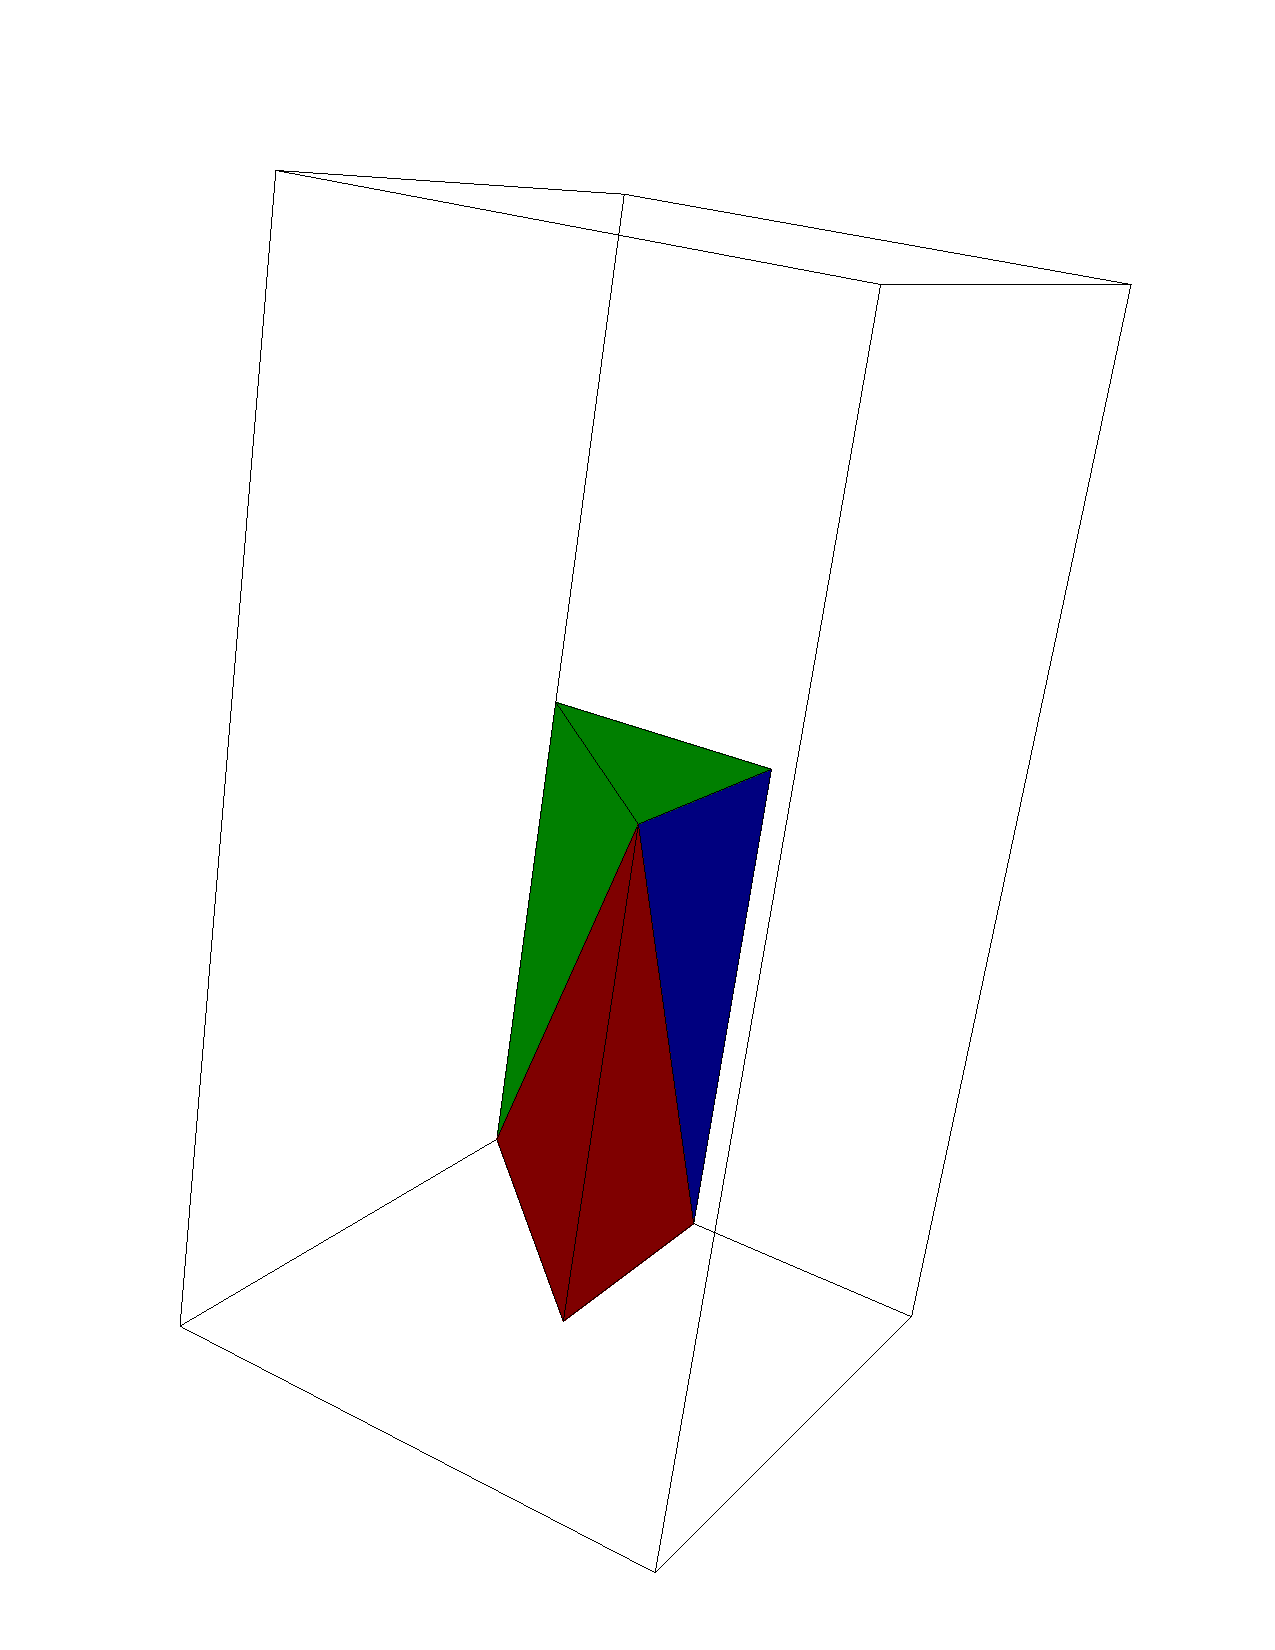
\includegraphics[width=0.4\textwidth]{hasab_bari.pdf}
    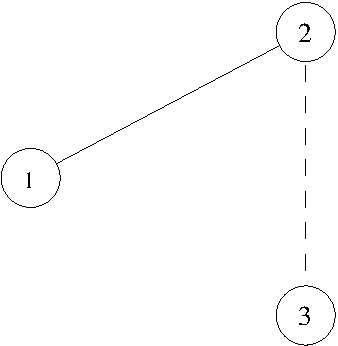
\includegraphics[width=0.35\textwidth]{hasab_D-graf.pdf}
  \end{figure}
  Notation:\\<all>
  \setlength{\unitlength}{1cm}
  $\sigma_0$:
  \begin{picture}(1,0.2)
    \multiput(0,0.1)(0.2,0){5}{\circle*{0.001}}
  \end{picture},
  $\sigma_1$:
  \begin{picture}(1,0.2)                                                                                 
    \multiput(0,0.1)(0.25,0){4}{\line(1,0){0.15}}                                                        
  \end{picture},
  $\sigma_2$:
  \begin{picture}(1,0.2)
    \put(0,0.1){\line(1,0){1}}
  \end{picture},
  $\sigma_3$:
  \begin{picture}(1.5,0.2)
    \multiput(0,0.1)(0.5,0){3}{\line(1,0){0.2}}
    \multiput(0.35,0.1)(0.5,0){3}{\circle*{0.001}}
  \end{picture}
\end{frame}

\begin{frame}
  $\mathcal{R}$ and $\mathcal{M}$ matrix-functions (where $\mathcal{D}$ is the set
  of simplex-orbits, $D_i\in\mathcal{D}$):
  \begin{equation*}
    \mathcal{R}(D_1)=
    \left(
    \begin{array}{cccc}
      1 & 1 & 2 & 1\\
      1 & 1 & 3 & 1\\
      2 & 3 & 1 & 2\\
      1 & 1 & 2 & 1
    \end{array}
    \right)
  \end{equation*}
  \begin{equation*}
    \mathcal{R}(D_2)=
    \left(
    \begin{array}{cccc}
      1 & 2 & 2 & 1\\
      2 & 1 & 3 & 2\\
      2 & 3 & 1 & 2\\
      1 & 2 & 2 & 1
    \end{array}
    \right)
  \end{equation*}
  \begin{equation*}
    \mathcal{R}(D_3)=
    \left(
    \begin{array}{cccc}
      1 & 2 & 1 & 1\\
      2 & 1 & 3 & 2\\
      1 & 3 & 1 & 1\\
      1 & 2 & 1 & 1
    \end{array}
    \right)
  \end{equation*}

  \begin{equation*}
    \forall D_i\in\mathcal{D}:\;
    \mathcal{M}(D_i)=
    \left(
    \begin{array}{cccc}
      1 & 4 & 2 & 2\\
      4 & 1 & 3 & 2\\
      2 & 3 & 1 & 4\\
      2 & 2 & 4 & 1
    \end{array}
    \right)
  \end{equation*}
\end{frame}

\section{Constraints for D-symbols}
The following constraints are needed for a D-symbol to have a corresponding
tiling.

\subsection{General constraints}
\begin{frame}
  D-symbol: $(\Sigma_I,\mathcal{D},\mathcal{M})$ triplets. \mode<article>{Where
  $I$ is the index set of the dimension ($|I|=dim+1$), $\Sigma_I$ is the set of
  adjacency operations (interpreted accordingly on the simplex-orbits and the
  simpleces), $\mathcal{D}$ is the set of simplex-orbits and $\mathcal{M}$ is
  the matrix-function on simpleces. These are the Delone-Delaney-Dress symbols,
  briefly D-symbols.}
  \begin{itemize}
    \item Natural constraints for D-diagrams:
      \begin{enumerate}
	\item $\mathcal{D}$ is finite
	\item Adjacency operations on simplex-orbits are involutive 
	  permutations\mode<article>{, this means $\forall i\in I, \sigma_i\in
	  \Sigma_I, \forall D\in \mathcal{D}$:
	  \begin{align*}
	    \sigma_i\sigma_i(D)=D 
	  \end{align*}
	  The degree of the uniformly colored edges in every vertice of the
	  diagram is $1$ or $2$. It is $2$ iff the edge is a loop.}
	\item Using not neighbouring operation-pairs we get back to the starting
	  vertice in at most $2$ steps\mode<article>{. \newline $\forall
	  i,j\in I, \forall D\in \mathcal{D}$:
	  \begin{align*}
	    |i-j|\geq 2 \Rightarrow (\sigma_j\sigma_i)^2(D)=D
	  \end{align*}}
      \end{enumerate}
    \item We can calculate the $\mathcal{R}$ matrix function\mode<article>{,
      which is the same for simplex-orbits as the $\mathcal{M}$ matrix function
      for simpleces: \newline $\forall i,j\in I, \forall D\in \mathcal{D}$:
      \begin{align*}
	r_{ij}(D)=r_{ji}(D)=\mathrm{min}\left\{r\in \mathbb{N}^+|(\sigma_j\sigma_i)^r(D)=D\right\}
      \end{align*}
      Constraints of the D-diagram on $\mathcal{R}$ matrix-function:
      $r_{ii}(D)=1$, and $|i-j|\geq 2 \Rightarrow r_{ij}(D)\leq2$}
    \item Constraints of the $\mathcal{M}$ matrix function:
      \begin{enumerate}
	\item Every element of $\mathcal{R}$ has to divide the appropriate
	  element of $\mathcal{M}$ (parameters)\mode<article>{. Because we have to get to the
	  same simplex walking around a $(d-2)$-dimensional face (which is an edge
	  in $3$ dimensions,) which means we have to get to the same
	  simplex-orbit too. The quotient of the elements of $\mathcal{M}$ and
	  $\mathcal{R}$ shows the periodicity of the tiling around the
	  $(d-2)$-dimensional face.
	  \newline $\forall i,j\in I, \forall D\in \mathcal{D}$:
	  $r_{ij}(D)|m_{ij}(D)$
	  }
	\item Orbits of adjacency-operation pairs\mode<article>{. An orbit can
	  be defined for every operation-pair and starting simplex-orbit
	  (diagram-vertex). Elements of $\mathcal{M}$ has to be the same inside
	  such an orbit. The reversed orbit has to contain the same number of
	  simpleces, so the matrices of $\mathcal{M}$ has to be symmetric.
	  \begin{align*}
	    &\forall i,j\in I, \forall D\in \mathcal{D} \\
	    &\mathcal{D}'=\left\{(\sigma_j\sigma_i)^k(D)|k\in
	    \mathbb{N}\right\}\cup\left\{\sigma_i(\sigma_j\sigma_i)^k(D)|k\in
	    \mathbb{N}\right\}\\
	    &\forall D_1,D_2 \in \mathcal{D}'\\
	    &m_{ij}(D_1)=m_{ij}(D_2)=m_{ji}(D_1)=m_{ji}(D_2)
	  \end{align*}
	  }
	\item The values of the main diagonal has to be $1$\mode<article>{,
	  because we have adjacency operations.}
	\item The values of the first diagonal above and below the main has to
	  be $\geq2$\mode<article>{. In case of equality we get
	  degenerated tilings, in which for example digons can be facets. (In
	  case of nice tilings in 3 dimensions every vertex joins at least 3
	  edges and 3 facets, every facet has at least 3 edges and every edge
	  joins 3 facets and 3 bodies.)}
	\item Every other value has to be exactly $2$\mode<article>{, so we stay
	  compatible with baricentric subdivision.}
	  $\forall i,j\in I, \forall D\in \mathcal{D}$:
	  \begin{align*}
	    i=j & \Rightarrow m_{ij}(D)=1 \\
	    |i-j| = 1 &\Rightarrow m_{ij}(D)\geq2 \\
	    |i-j|\geq2 &\Rightarrow m_{ij}(D)=2
	  \end{align*}
      \end{enumerate}
  \end{itemize}
\end{frame}

\subsection{$2$-dimensional subtilings I.}
\begin{frame}
  From now on we only consider $3$-dimensional D-symbols. \newline
  D-subsymbol:
  \begin{itemize}
    \item The $i$-th D-subsymbol 
      $(\Sigma_I^i,\mathcal{D}^i,\mathcal{M}^i)$\mode<article>{ can be got by
      eliminating the $i$-th operation from the diagram and the rows and columns
      of the matrix functions.}
    \item We can calculate the combinatorial curvature function of the subsymbol:
      \begin{align*}
	K(\leftexp{c}{\mathcal{D}}^i)=\sum_{D\in
	\leftexp{c}{\mathcal{D}}^i}\left(-1+\sum_{\substack{0\le j<k\le d \\
	j,k\ne i}}\frac{1}{m_{jk}(D)}\right)
	\begin{array}{cccc}
	  > & & S^2 \\
	  = & 0 & \mathbb{E}^2 \\
	  < & & H^2
	\end{array}
      \end{align*}
      \mode<article>{Based on the above formula one can decide, in which
      $2$-dimensional constant curvature space realizes the tiling.}
  \end{itemize}
  \mode<presentation>{\begin{minipage}[t]{0.45\textwidth}}
    \begin{itemize}
      \item Good orbifold criteria\mode<article>{: In the above mentioned
	spherical tiling case, we have to exclude bad orbifolds. The following
	options are excluded (given by both Convay's and Macbeath's notations):
	\begin{align*}
	  u=(+,0;[u];\{\}), & & 1<u;\\
	  *u=(+,0;[];\{(u)\}), & & 1<u;\\
	  uv=(+,0;[u,v];\{\}), & & 1<u<v;\\
	  *uv=(+,0;[];\{(u,v)\}), & & 1<u<v.
	\end{align*}}
      \item Visualization:
	\mode<article>{The subsymbol corresponds to the $(3-1)$-dimensional
	tiling around the $i$-indexed vertice-class inducated by the
	original D-symbol. So we have to get a spherical tiling around a real
	simplex-vertice (see Fig. \ref{fig:spherical_ex}), or a Euclidean tiling
	around an ideal simplex-vertex in the original tiling. We should not get
	hyperbolic tilings around a simplex-vertex, because this would mean an
	out-of-model vertex.}
    \end{itemize}
  \mode<presentation>{\end{minipage}
  \begin{minipage}[t]{0.5\textwidth}}
    \begin{figure}
      \mode<article>{\caption{\label{fig:spherical_ex}Spherical tiling around
      a simplex-vertex}}
      \center
      \includegraphics[height=2.5cm]{d3c3_2_vertice.pdf}
    \end{figure}
  \mode<presentation>{\end{minipage}}
\end{frame}

\begin{frame}
  Further constraints in $3$-dimensional D-symbols based on $2$-dimensional
  subsymbols:
  \begin{enumerate}
    \item For $(\Sigma_I^1,\mathcal{D}^1,\mathcal{M}^1)$ and
      $(\Sigma_I^2,\mathcal{D}^2,\mathcal{M}^2)$ the combinatorial curvature
      function has to be positive and the tiling has to be good
      orbifold\mode<article>{. Edge- and face-centered simplex-vertices has to
      be real vertices, so the tiling around them has to be an $S^2$ tiling.}
    \item For $(\Sigma_I^0,\mathcal{D}^0,\mathcal{M}^0)$ and
      $(\Sigma_I^3,\mathcal{D}^3,\mathcal{M}^3)$ the combinatorial curvature 
      function has to be non-negative, and if positive the tiling has to be good
      orbifold\mode<article>{. Vertex- and body-centered simplex-vertices can be
      real or ideal vertices, so the tiling around them can be an $S^2$ or an
      $\mathbb{E}^2$ tiling. (We do not exclude ideal body-centers because of
      the duality.)}
  \end{enumerate}
  These constraints lead to an upper bound of the parameters \mode<article>{as a
  system.}
\end{frame}

\subsection{$2$-dimensional subtilings II.}

\begin{frame}
  \frametitle{Splitting problem and the Thurston conjecture}
  Thurston conjecture:
  \begin{itemize}
    \item Every oriented prime closed 3-manifold can be cut along tori, so that
      the interior of each of the resulting manifolds has a geometric structure
      with finite volume.
    \item There are 8 possible geometric structures in 3 dimensions, which have
      at least one compact manifold modelled on itself: $S^3$, $E^3$,
      $H^3$, $S^2\times R$, $H^2\times R$, $\widetilde{SL2R}$, Sol,
      Nil.
  \end{itemize}
  Remarks:
  \begin{itemize}
    \item For non-orientable manifolds the "oriented double cover" method can be
      used\mode<article>{. Which maps manifold $M$ to $M\times Z/2Z$ with an
      appropriate pull-back operation. For example a Möbius-strip is mapped to a
      "double Möbius-strip" which is a ring.}
    \item In $2$ dimensions: every surface without boundary (2-manifold) has a
      geometric structure consisting of a metric with constant curvature
  \end{itemize}
\end{frame}

\begin{frame}
  Finding splittings in a D-symbol
  \begin{itemize}
    \item $S^2$-type splitting: Indicates a detail in the tiling, which is
      shrinkable to a single vertex, so we get a similar tiling \mode<article>{ with
      less simplex-vertices, so} with less simplex-orbits. (Possible bad
      orbifold problem.) \mode<article>{(See fig. \ref{fig:s2splitting}.)}
      \begin{figure}
	\mode<article>{\caption{\label{fig:s2splitting} $S^2$-type splitting}}
	\center
	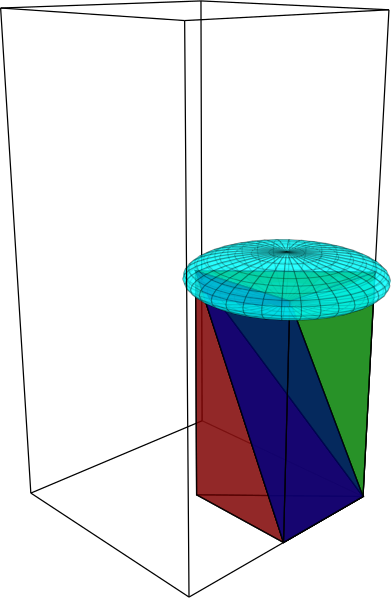
\includegraphics[height=2.5cm]{d3c3_2_splitting1.pdf}
      \end{figure}
    \item $E^2$-type splitting: In Thurston-conjecture "cut along tori". This
      indicates two parts in the tiling, in both parts the other part
      can be seen as an ideal vertex. \mode<article>{There are at least 3
      possible combinations, from which only the first one indicates a
      splitting, the second one most likely indicates a fibration and the third one
      is not possible, because inside the torus there is a full $2$-dimensional
      plane. (See fig. \ref{fig:e2splitting}.)}
      \begin{figure}
	\mode<article>{\caption{\label{fig:e2splitting} $E^2$-type splittings}}
	\center
	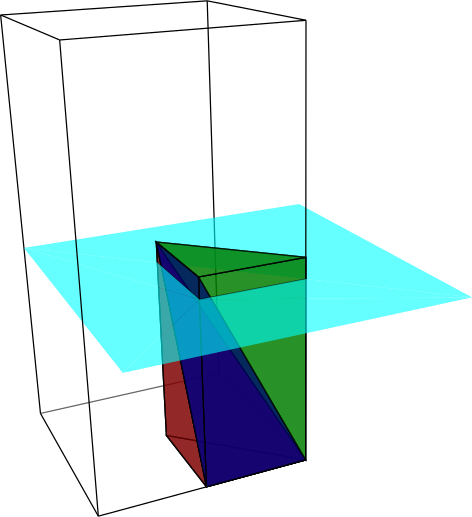
\includegraphics[height=2.5cm]{d3c3_2_splitting2_alt1.pdf}
	\hspace{0.1\textwidth}
	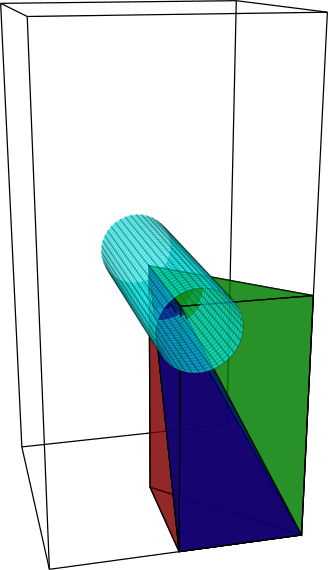
\includegraphics[height=2.5cm]{d3c3_2_splitting2_alt2.pdf}
	\hspace{0.1\textwidth}
	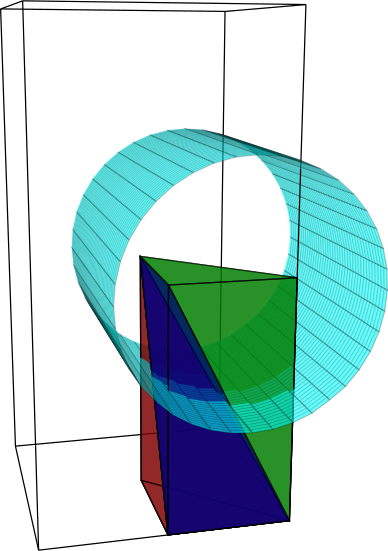
\includegraphics[height=2.5cm]{d3c3_2_splitting2.pdf}
      \end{figure}
  \end{itemize}
\end{frame}

\begin{frame}
  Further constraints for tilings without splittings
  \begin{itemize}
    \item The above figures and remarks show that if we calculate the
      combinatorial curvature function for the appropriate $2$-dimensional
      tilings, we can get a lower bound for the parameters.
    \item Based on the $3$-dimensional D-diagram, we can describe the tiling's
      simplex-vertices and the edges between simplex-vertices. Take this system
      as a graph, we have to examine every possible 2-partitions (where both
      partitions have at least 2 vertices).
    \item If we examine every such "splitting-candidates", we can get every
      lower bound for the parameters.
    \item Such D-symbols do not have $E^2$ nor $S^2$ splittings. (If we could
      find one such that it's not realizable in any of the 8
      Thurston-geometries, then this would be a counter-example of the Thurston
      conjecture.)
  \end{itemize}
\end{frame}


\section{Enumerating D-symbols}
\begin{frame}
  Enumerating D-symbols
  \begin{itemize}
    \item Ambitious goal\mode<article>{: Let's enumerate every possible
      $n$-dimensional tiling with compact fundamental domain using D-symbols.}
    \item It may be possible\mode<article>{, because we can define D-symbols for
      every tiling that has "finite" baricentric subdivision.}
    \item Too many cases\mode<article>{: the output is exponential both in the
      dimension and the cardinality of the D-diagram.}
    \item There is an ordering on D-diagrams, so they can be enumerated
    \item There is an ordering on matrix-functions, we can enumerate them in $3$
      dimensions\mode<article>{. Based on the previous sections there is an
      upper bound on parameters (but one has to be cautious, because there are
      infinite chains.) We do not use the lower bounds yet.}
    \item Our algorithms could enumerate the $3$-dimensional D-symbols with
      cardinality at most $12$.
  \end{itemize}
\end{frame}

\subsection{Enumerating edge-transitive D-symbols}
\begin{frame}
  How can we use the D-symbols for $3$-dimensional edge-transitive tilings?
  \begin{itemize}
    \item Very simple new constraint: the D-diagram cannot "fall apart" if we
      cancel it's $1$-colored (dashed) edges
    \item Let's enumerate diagrams without $1$-colored edges, and put back them
      in every possible (good) way
    \item Enumerating diagrams becomes easier
    \item Our algorithms could enumerate these D-symbols with cardinality at
      most $18$, and it can be proved that the maximal cardinality of such
      tilings is $24$
  \end{itemize}
\end{frame}

\begin{frame}
  \nocite{DHM93,D87,Du88,H93,LM90,Ma67,M94,T82,VS93,F94,F03}
  \bibliographystyle{plain}
  \mode<presentation>{\fontsize{5pt}{0}}
  \bibliography{dsym}
\end{frame}

\end{document}
